% -*- coding: utf-8 -*-
\documentclass[a4paper,10pt]{article}
\usepackage[english]{babel}
\usepackage{graphicx}
\usepackage{textcomp}
\usepackage{hyperref}
\usepackage{makeidx}
\usepackage{url}
\usepackage{listings}
\usepackage{amsmath}
\usepackage{pslatex}
\usepackage[utf8]{inputenc} 
\usepackage{xspace}
\usepackage{bnf}

% variable definition
%%%%%%%%
\newcommand{\aadl} {\textsc{AADL}}
\newcommand{\real}{\textsc{REAL}}
\newcommand{\ocarina}{\textsc{Ocarina}}


% Support syntax highlighting for REAL

\lstdefinelanguage{real}
{morekeywords={theorem, foreach, in, do, check, end, requires, |},
   morekeywords= {and, or, not}, 
   morekeywords= {if, then, else}, 
   morekeywords= {T_Data, T_Subprogram, T_Subprogram_Call, T_Sequence_Call, T_Thread, T_Threadgroup, T_Process, T_Memory, T_Processor, T_Bus, T_Connection, T_Device, T_System},
  morecomment=[l]{--},
}

% Layout for listings

\lstset{language=real,
        basicstyle=\scriptsize\sffamily,
        aboveskip=.1cm, % \smallskipamount, % \bigskipamount,
        belowskip=.1cm, % \smallskipamount, % \bigskipamount,
        abovecaptionskip=.1cm, % \smallskipamount, % \medskipamount,
        belowcaptionskip=.1cm, % \smallskipamount, % \bigskipamount,
        xleftmargin=.0cm,
        captionpos=b,
        tabsize=3,
        numberstyle=\tiny, 
        frame=single,
        }

% Support syntax highlighting for AADL

\lstdefinelanguage{aadl}
{morekeywords={in,out,package,end,bus,data,thread,port,group,process,processor,
system,memory,device,subprogram,public,private,event,property,set,applies,to,
units,type,implementation,parameter,reference},
  morekeywords={properties,features,annex,modes,connections,flows,
  subcomponents,calls,binding},
  morekeywords={aadlinteger,aadlboolean,aadlstring,aadlfloat},
morecomment=[l]{--},
}

% Layout for listings

\lstset{language=aadl,
        basicstyle=\scriptsize\sffamily,
        aboveskip=.1cm, % \smallskipamount, % \bigskipamount,
        belowskip= \smallskipamount, % \bigskipamount,
        abovecaptionskip=-.5cm, % \smallskipamount, % \medskipamount,
        belowcaptionskip=.0cm, % \smallskipamount, % \bigskipamount,
        xleftmargin=.0cm,
        captionpos=b,
        tabsize=3,
        }


%opening

\title{
  \textbf{REAL : Requirement Enforcement Analysis Language}
}

\author{Olivier GILLES}

\begin{document}

\maketitle
\newpage
\tableofcontents
\newpage

\section {About This Document}

This document aims to present \real{}, a language for requierements
expression on architectural language.

\subsection {What This Guide Contains}

This document contains the following sections:
\begin {itemize}

\item section~\ref{Intro} provides a brief description of the issues 
that \real{} aims to address and compare it to existing works on 
related subjects;

\item section~\ref{aadl_descr} provides a bried description of the 
architectural language \aadl{} and the tool that we use in order to 
manipulate it, \ocarina{};

\item section~\ref{language_description} provides a proposition of 
language in order to describes thoses verifications;

\item section~\ref {examples} describes some examples of hardware 
verification;

\item section~\ref {predefined} describes more precisely the 
predefined functions and sets.
\end {itemize}


\section{Motivations}
\label {Intro}

In this section, we present the place of non-functional requirements
definition within the software development process and then the works
related to non-functional requirement definition and verification.

\subsection {Introduction}

Distributed Real-time and Embedded (DRE) systems must enforce
constraints of both the real-time and embedded domains. They need to
comply with specific requirements: strict determinism, low resource
consumption and reliability.

Designing DRE systems is a complex and thus expensive task, which
requires highly specialized manpower. Some methodologies have been
developed in order to reduce DRE development costs, amongst them,
model-driven design (MDD) coupled with code generation appear to be
one of the most promising in reducing the development cost and
increasing reliability.

DRE systems must enforce a large set of non-functional requirements
that come from their versatile nature. A real-time application needs
strong timing guarantees; a distributed one must not break those
guaranties. An embedded application also needs to check resource
usage. Hence, enforcement of non-functional requirements is required
to assess DRE system consistency. Yet, the complexity of expression 
of these constraints is directly proportional to the level of
restrictiveness of the non-functional requirements.

Therefore, one need an efficient way to express these requirements on
the model prior to evaluating them. One need also to make sure there
is no divergence between the model and the requirements put on this
model.

In this document, we present a solution to these two problems for
AADL-centric processes, using a Domain Specific Language. This DSL
checks non-functional constraints at model level, ensuring that the
model is ready for further analysis (e.g. schedulability) or code
generation for constrained run-times.

\subsection{Software development process}

The software development process maps requirements onto high-level,
low-level and code-source level descriptions. At each level,
functional and non-functional requirements must be refined, faithfully
translated to the actual system description, and also preserved. Some
of them can be also checked at each stages.

Architecture Description Languages (ADLs)~\cite{medvidovic97framework}
aim at describing the system architecture. An ADL-based development
process consists of modeling the application, analyzing it and then
generating source code. ADL toolsuites can also provide support for
describing system requirements for further validation and
verification. Some examples of such approach are STOOD~\cite{stood},
OSATE~\cite{osate} and TOPCASED~\cite{topcased}.

DRE systems have complex non-functional requirements. While some of
them are generic (and solved using well-known design patterns, e.g.
concurrency~\cite{douglass2002real-time-desig}), most of them are
highly application-dependent. Hence, it is necessary to have a
language which can express application requirements. ADLs can document
low-level architectures, but not constraints on them. Therefore,
defining a language as a Domain Specific extension of an ADL would
enable one to describe both software architecture and requirements in
the same model. A checker for this language would validate model
conformance to these requirements. This would simplify code generation
from specific ADL patterns.

\subsection{Related work}

Non-functional requirements definition and enforcement can be
performed by adding constraints to the
model. UML~\cite{omg2003uml-2.0-superst} and its derivatives
(MARTE~\cite{omg2007a-uml-profile-f}) are the de jure standards.
Object Constraint Language~\cite{OCL98} (OCL), is a standard to
express constraints on UML models. OCL constraints are described over
the concepts of a meta-model and evaluated over a model which is an
instance of the meta-model.  OCL requires a generic API to express
queries, leading to complex expressions for assessing details of a
model. This indirection to a higher level of abstraction increases the
learning curve.

Approaches exist to map a model onto other formalisms for verification
purposes, e.g. using algebraic approaches like Z for modeling
RT-POSIX~\cite{f06}; or model checking techniques for verifying
RT-CORBA middleware using the Bogor model checker~\cite{bogor}. Yet,
this introduces a new modeling space to master, especially for domain
engineers. One need to automate the mapping between these two
spaces. Besides, it could introduce inconsistencies in the process
when one model is updated, but not the other. This could lead to
inadequate or incomplete models. Therefore, one need to add
requirements directly on the model to ensure analysis techniques are
still applicable, and that the requirements apply to an up-to-date model.

Therefore, we propose a DSL mapped to the concept of meta-model, while
being simple enough to reduce risk of inconsistency and learning
time. Using mathematical notations from set theory would make this
language easier to manipulate. In this paper, we present a solution
and its implementation on top of the \aadl{}. \aadl{} already has
supporting tool for schedulability analysis, code
generation. Complementing it with a DSL for specifying constraints
would ensure \aadl{} models are ready for being processed by such
tools in a transparent way.

\section{Short overview of \aadl{} and \ocarina{}}
\label{aadl_descr}

\aadl{} (\textit{Architecture Analysis and Description
  Language})~\cite{aadl-v1.0} aims at describing DRE systems by
assembling components. \aadl{} allows for the description of both
software and hardware parts of a system. It focuses on the definition
of interfaces, and separates the implementations from these
interfaces.

An \aadl{} description is made of \emph{components}.  The \aadl{}
standard defines software components (\texttt{data}, \texttt{thread},
\texttt{thread group}, \texttt{subprogram}, \texttt{process}) and
execution platform components (\texttt{memory}, \texttt{bus},
\texttt{processor}, \texttt{device}) and hybrid components
(\texttt{system}). Components describe well identified elements of the
actual architecture. \emph{Subprograms} model procedures as in C or
Ada. \emph{Threads} model the active part of an application (such as
POSIX threads). \aadl{} threads may have multiple operational
modes. Each mode may describe a different behaviour and property
values for the thread. \emph{Processes} are memory spaces that contain
the \emph{threads}. \emph{Processors} model micro-processors and a
minimal operating system (mainly a scheduler). \emph{Memories} model
hard disks, RAMs, \emph{buses} model all kinds of networks, wires,
\emph{devices} model sensors, etc.

An \aadl{} model also describe non-functional facets: embedded
or real-time characteristics of the components (execution time, memory
footprint\ldots), behavioral descriptions, etc. Description can be
extended either through new property sets, or through annexes. Annexes
are extensions to the core language. A complete introduction to the
\aadl{} can be found in~\cite{feiler06aadl}.

\begin{figure}[h]
\centering
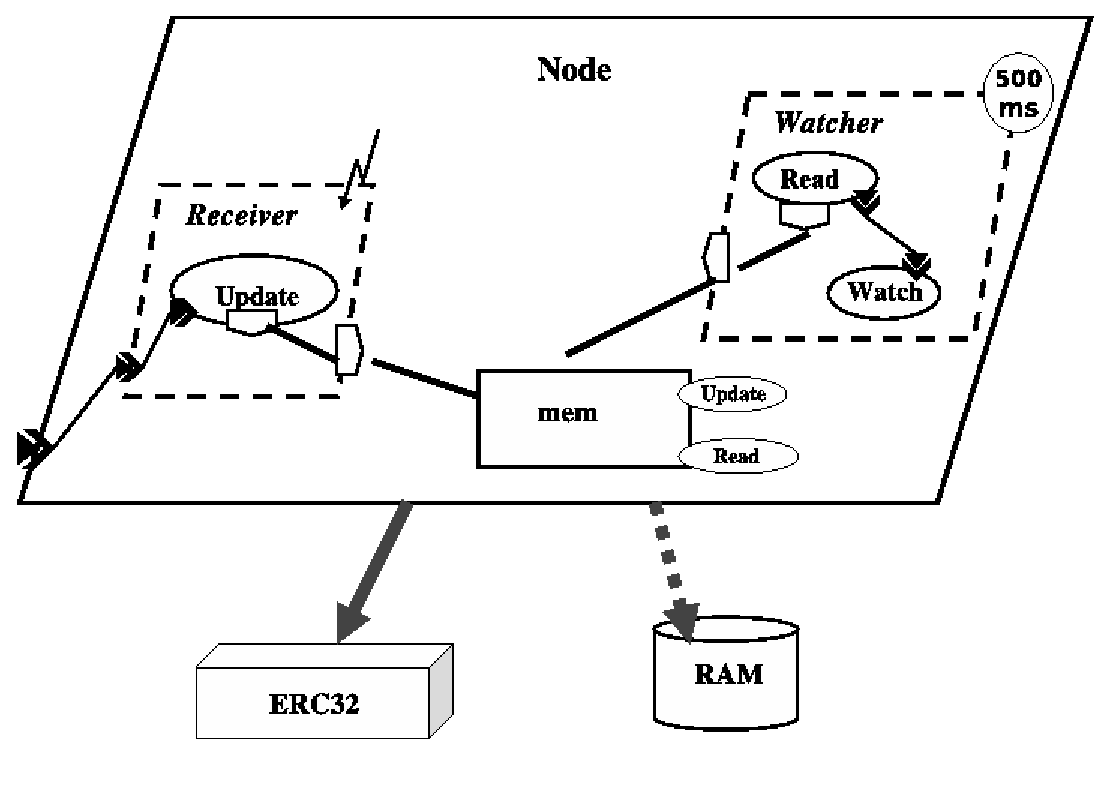
\includegraphics[height=6cm]{figs/figure-aadl-v4.eps}
\caption{Sample \aadl{} model}
\label {case_study}
\end{figure}

Figure~\ref{case_study} is a sample \aadl{} model.  It models two
threads: one periodic and one aperiodic that interact to read and update
a shared variable. Both threads are subcomponent of a process,
bound to a processor and memory.

We have developed the \ocarina{}~\cite{enst06ocarina} toolsuite to
manipulate \aadl{} models. \ocarina{} proposes \aadl{} model manipulation
based on a compiler-like API. ``Back-end'' modules can generate
formal models, perform scheduling analysis and generate
distributed high-integrity applications in Ada.

Generated code relies on the PolyORB-HI~\cite{HZP06} middleware to
ensure communications and task allocation. PolyORB-HI ensures that a
minimal and reliable middleware is generated for a given distributed
application.

\aadl{} is a complete ADL that describes in -depth the architecture of
a system. It allows for layered design through component
refinement. Besides, the designer can express all is non-functional
requirements.  We now detail how we enriched \aadl{} with a DSL to
check non-functional properties at model level.

\section {REAL basic constructs}
\label  {language_description}

\real{}\footnote {REAL sources and documentation can be accessed 
from http://aadl.enst.fr/ocarina/real.html} (Requirement Enforcement 
Analysis Language) aims at checking adequacy between different parts 
of architectural descriptions, with emphasis on conciseness and 
simplicity. In this section, we describe the main features of this 
language.

\real{} is based on set theory. It allows one to build sets whose
elements are \aadl{} entities (connections, components or subprogram
calls). Verification can then be performed on either a set or its
elements by stating Boolean expressions. The basic unit of \real{} is
a \textit{theorem}. A theorem is made of 3 parts :
\begin {itemize}
\item range definition;
\item destination set building;
\item verification expressions. 
\end {itemize}
In the following subsections, we review each of them.

\subsection{Range definition}

The \textit{range definition} selects the class of component instances
on which the verification must be done. All following declarations
(either set building or verification expressions) are performed for
each element of the range set. An element of the range set is a
\textit{range variable}.

\lstset{language=aadl}
\lstinputlisting[caption=\aadl{} threads, label=aadl_example_data]
                {sources2/data.aadl}

Listing~\ref{aadl_example_data} is an excerpt of the \aadl{} model in
figure~\ref{case_study}.  In this example, let us assume that a range
set is declared as being formed of the predefined thread set.

\lstset{language=real}
\lstinputlisting[caption=Thread periodicity, label=thread_decl]
                {sources2/range_set.real}

In this case (listing~\ref{thread_decl}), the range
variable \textit{e} would be successively valued as
the first thread (\textit{Receiver}) in the first
evaluation iteration, then to the second one
(\textit{Watcher}).

\subsection{Destination set building}
\label{set_building}

\textit{Destination set building} defines sets that can refer to
previously-defined ones. Additionally, they can refer to predefined
sets (canonical one, e.g. all processors in a model). Their elements
can be declared to be compliant to certain properties. These definitions
(or \textit{relations}) are defined this way: \texttt{S
  $:=$ {x in E | f (x)}}, where the character '\texttt{|}' is an 
abbreviation for \texttt{such as}. In \real{}, it means that the 
destination set will be formed by all elements of the set \texttt{E}
which verify the expression \texttt{f(x)} (which is an application 
from the set E to the boolean).

This means that \texttt{S} holds all the elements of the set
\textit{E} that comply with the relation \textit{f}. Hence, set
building is done by giving its first-order logic definition.

\lstset{language=aadl}
\lstinputlisting[caption=\aadl{} protected data,
  label=aadl_example_data_def]
                {sources2/data_def.aadl}

Let us suppose we want to build the set of concurrency-safe data
(i.e. for which the \aadl{} property
\textit{Concurrency\_Control\_Protocol} is set
(listing~\ref{aadl_example_data_def})). The set of concurrency-safe
data components is~:

\lstset{language=real}
\lstinputlisting[caption=access-protected set building]
                {sources2/set_building.real}
\label{set_building_real}

Note that the expression that each element must complies to (ie. 
the \textit{selection expression}) is build in the same way as the
\textit{verification expression}, but actually uses \textit{relations}
in addition to regular function. Explanation about relation usage can 
be found in~\ref{relation_def}.

\subsection{Verification expression}

\textit{Verification expressions} check properties on sets,
according to the range variable. If it refers to the range
variable, or if it refers to any set that refers to the the range
variable, it will be evaluated for each element of the range set.

For listing~\ref{aadl_example_data}, one might want to check whether
all threads are periodic. Using the check in listing~\ref{period}, the
evaluation will fail on the first element \textit{e} (the
\textit{Receiver} thread), but would have been successful on the
second one (the \textit{Watcher} thread).

\lstset{language=real} \lstinputlisting[caption=Thread periodicity,
  label=period] {sources2/evaluation.real}

An alternative to \textit{verification expression} is \textit{return 
expression}. It is basically build with the same rules, but the 
top-level expression type after resolution must be real instead of 
boolean. A complete description of both expression building rules
can be found in~\ref{expression_def}.

\section {REAL features}

\subsection {theorems}

% -*- coding: utf-8 -*-

\label {theorems}

\paragraph{}
A requierement or constraint can be describe in a \real{} 
\textit{theorem}. A theorem is a named entity which can be compared 
to a subprogram, which can return either a boolean value (if it 
finish with a \textit{verification expression}) or a real value (if it 
finish with a \textit{return expression}). It can be called directly 
by our parser/interpreter, or called by other theorems, eventually 
with parameters.

\subsubsection {Sub-theorem calls}

A theorem can be called by another theorem by two ways :
\begin{itemize}
\item using the keyword \texttt{compute};
\item using the keyword \texttt{requires};
\end{itemize}
In the first case, the theorem called (ie. the \textit{subtheorem})
must return a numeric (real or integer) value. Otherwise, it must 
return a boolean value.

\subsubsection {Parameters}

While called with \texttt{compute}, a subtheorem can be assigned 
parameters of any types, and a domain (a set or an element). Assigning 
a domain will overwrite the local set. In the subtheorem, the 
parameters can be accessed with \texttt{argv\_i}, where \texttt{i} is 
the number of teh parameter, up to 10. 

Note that using a parameter in an expression will make pre-execution 
analysis impossible, as parameter type are only known at run time.

\subsubsection {Contextued theorems}

The normal way to define a theorem is a REAL file. Nevertheless, this 
only allows to run theorems on the whole model, or on all components
verifiying a given expression of the model. In some case, such 
solution is not acceptable, for it could be needed to run a theorem
on all the instances of a component and no others. It is the case when 
some components have unique limitations (eg., heterogenous hardware
components).

In order to address this issue, a theorem can be defined within an 
\aadl{} component annex. In this case, the \textit{local set} will 
contains all instances of this component. Whenever a contextued theorem
call another theorem with the \texttt{requires} keyword, the subtheorem 
inherit the caller local set.


\subsection {Sets}

\subsubsection {Set definition}
\paragraph{}
Lets $S_1$, $S_2$ ... $S_N$ be pre-defined sets of instances. 
All pre-defined sets are typed according to the AADL instance 
types they are coming from.

eg. :

\textit{Process\_Set} is the set which contains all processes 
instances.

\subsubsection {Set functions}
\label {set_operations}

\paragraph{}
In some case set must be restricted or joined in order to build 
the final set. Set operations are defined in the sets space (ie. 
they takes sets as arguments and returns sets). Set functions are
called within set expressions (cf~\ref{expression_def}).

eg. : 

\textit{Union} is a function which take two sets and returns 
the sets resulting in the union of the two sets, with delete 
equal elements (ie. if an element is at the same time in E1 
and E2, it is present twice in the result of Union (E1, E2).

\subsubsection {The \textit{local} set}

\paragraph{}
If a theorem is defined within a AADL composant annex or if it is 
called with a specified \textit{domain} then the \textit{local} set 
is defined. Note that \textit{Local\_Set} is a valid set expression.

\subsubsection{Relations}
\label {relation_def}

As exposed in Section~\ref{set_building}, sets can be defined that
refer to previously defined sets. Sets gather elements matching
specified properties. \real{} defines relations to find hierarchical
links between \aadl{} component instances. Relations allow to navigate
in the \aadl{} model and thus to access \aadl{} architectural
semantics within \real{}. For instance, the relation \texttt{A
  is\_subcomponent\_of B} returns \texttt{true} whenever the
instance A is a subcomponent of the instance B.  Relation can be
expressed between two elements, or between a set and an element. In
that case, this example would return true whenever A is a subcomponent
of any element of the set B. All existing relations are presented in
section~\ref{predefined_stuf}.



\subsection {Types}
\label {types}


\paragraph{}
REAL supports two main kind of data :
\begin {itemize}
\item sets
\item elements
\end {itemize}
Sets and elements may be typed, in order to reduce 
errors. 

\subsubsection {Elements}
\paragraph{}
An element ``T\_Generic'' , or within the list of 
types supported :
\begin {itemize}
\item T\_Data
\item T\_Subprogram
\item T\_Subprogram\_Call
\item T\_Sequence\_Call
\item T\_Thread
\item T\_Threadgroup
\item T\_Process
\item T\_Memory
\item T\_Processor
\item T\_Bus
\item T\_Connection
\item T\_Device
\item T\_End\_To\_End\_Flow
\item T\_System
\end {itemize}
All types corresponding to an existing AADL instance type.

\paragraph{}
An element typed as T\_Generic does not lose its original 
type, but is still considered as T\_Generic as far as 
comparisons are needed.

\subsubsection {Sets}
\paragraph{}
A set type is the type of the elements it can have. Any 
attempt to add an element of different type would lead 
to an error return.

\paragraph{}
The T\_Generic type can replace any type, which means 
that a set typed as T\_Generic can contain any type 
of elements. An element extracted from a T\_Generic set
will be considered as T\_Generic, no matter what is its
actual AADL type.


\subsection {Variables}

\label {variable_def}

\real{} allows to declare variables of tree different scopes :
\begin {itemize}
\item global scope;
\item theorem scope;
\item local scope.
\end {itemize}
The two first kind of variables are declared in the same place as 
theorem's sets, while the latter is declared within expression with
the keyword \texttt{expr}.

\subsubsection {Global an theorem variables}

Global and theorem variables are declared either by associating them
with sub-theorem calls or to expression. In the first case, the 
declaration part with begin by the keyword \texttt{compute}. In the 
latter case, no special keyword need to identify the association as 
such.

Global scope variables are declared with the \texttt{global} keyword, 
while theorem scope variables are declared with the \texttt{var} 
keyword.

A theorem scope variable will be visible from any latter part of the 
theorem. A global scope variable will be visible from any latter part 
of the theorem, and from any part of teh sub-theorems called with 
\texttt{compute}.

\subsubsection {Local variable}

A \textit{local variable} is a variable bind to a specific set. A 
local variable does not need to be explicitely declared, since it is
implicitely declared in the \texttt{expr} parameters.

The keyword \texttt{expr} allows to bind a local variable to a set, 
and to compute an expression according to each value of the set.
Its tree parameters are in order :
\begin {itemize}
\item An existing set name;
\item A non already existing variable name;
\item An expression.
\end {itemize}
The expression specified as third parameters can refer to the variable
name passed as first parameter. At run-time, the value of the expression
while be computed for any value of the variable which is defined in the 
parameter-passed set, and returned as a list of value. A local scope 
variable is only visible whitin the expression specified as third 
parameter. 

\subsection {Expressions}

%FIXME
\label {expression_def}

\paragraph{}
\real{} use expressions in order to perform any computation associating
sets, literals and function. Their is two kind of expressions : \textit{set 
expressions}, which take sets or set expressions as operands and return a
set, and \textit{regular expressions}, or \textit{expressions}, which take
sets, literals, variables or functions as operands and returns a value or 
a list of values. This section explains all expressions building.

\subsubsection {Set Expression}

\textit{set\_expression} $:=$ $<$declared\_set$>$ $|$ \textit{set\_expression} \textit{set\_operator} \textit{set\_expression}

\textit{set\_operator} $:=$ \textbf{+} $|$ \textbf{*} $|$ \textbf{/}

\paragraph{Operators}
\begin {itemize}
\item \textbf{+} : Union (x in A or x in B)
\item \textbf{*} : Intersection (x in A and x in B)
\item \textbf{/} : Exclusion (x in A and not x in B)
\end {itemize}

\subsubsection {Regular Expression}

\textit{expression} $:=$ $<$literal$>$ $|$ $<$variable$>$ $|$ $<$suprogram\_call$>$ $|$ \textit{expression} \textit{operator} \textit{expression}

\textit{operator} $:=$ \textbf{+} $|$ \textbf{*} $|$ \textbf{/} $|$ \textbf{and} $|$ \textbf{or} $|$ \textbf{not} $|$ \textbf{$<$} $|$ \textbf{$<=$} $|$ \textbf{$>$} $|$ \textbf{$>=$} $|$ \textbf{=} $|$ \textbf{**} 

\paragraph{Operators}
A check expression real type (ie. after evaluation) can be either 
boolean, real, integer, string, of a list of any of those types. 
Lists are handled by functions ratehr than by operators, and thus 
are addressed in section~\ref{check_function}.\\
Note that the top-level check expression must be a boolean.
\begin {itemize}
\item \textbf{+} : addition, defined on reals and integers;
\item \textbf{-} : substraction, defined on reals and integers;
\item \textbf{*} : multiplication, defined on reals and integers;
\item \textbf{**} : power, defined on reals and integers (second parameter must be integer);
\item \textbf{and} : and (x complies to A and x complies to B), lazy operator;
\item \textbf{or} : or (x complies to A or x complies to B), lazy operator;
\item \textbf{not} : not Exclusion (x does not comply to A);
\item \textbf{$>$} : strictly greater, defined on reals and integers;
\item \textbf{$<$} : strictly less, defined on reals and integers;
\item \textbf{$>=$} : greater or equal, defined on reals and integers;
\item \textbf{$<=$} : less or equal, defined on reals and integers;
\item \textbf{$<>$} : different (not equal), defined on reals, integers, strings and booleans;
\item \textbf{=} : equal, defined on reals, integers and strings;
\end {itemize}

\subsubsection {Ternary Expression}

\textit{ternary\_expression} $:=$ \textbf{if} \textit{boolean\_expression} \textbf{then} \textit{expression} \textbf{else} \textit{expression}

The ternary expression is typically used to perform conditional 
assignation, generaly used in conjonction with a variable assignation :

\textbf{var} \textit{variable\_name} $:=$ \textbf{if} \textit{boolean\_expression} \textbf{then} \textit{expression\_1} \textbf{else} \textit{expression\_2}

where \textit{variable\_name} contains \textit{expression\_1} if \textit{boolean\_expression} is true, and textit{expression\_2} if it is false.

\subsubsection {Expression and theorems type}

The regular expression specified after the keywords \texttt{check} 
or \texttt{return} is applied to all the elements of the range set.

If the theorem finish with \texttt{check}, then it is considered 
false if at least one element of the range set does not comply to 
the expression, which must return a boolean value.

If the theorem finish with \texttt{return}, then the value 
returned by the theorem is the value returned by the expression,
which must be a numeric. The result is always casted to a real. Note
that if the result of the expression is a list of values, one can use
an \texttt{aggregation function} on it. Existing \texttt{aggregation 
function} are \texttt{MSum} and \texttt{MMax}, which respectively 
returns the list's sum and maximum values. Of course, they are defined 
only on lists of numeric values.

\textit{return\_expression} $:=$ [$<$aggregation\_subprogram$>$ (]  \textit{expression} [)]


\subsection {Keywords}
%FIXME : update
\paragraph{}
This section explains all keywords meaning and usage.

\subsubsection {in}
\paragraph{}
Usage :\\
$<$Element\_Name\_A$>$ \textbf{in} \textit{Set\_Expression}\\

\paragraph{}
Defines the element Element\_Name\_A as being an element of the 
set resulting in Set\_Expression.\\
An element of a set can be declared in two moment : 
\begin {itemize}
\item when declaring verification range~\ref{range}, in which case 
this element will be used as a variable either in the buffer set 
definition or in the actual verification~\ref{verif};
\item when defining a set with the syntax x \textbf{in} E 
\textbf{|} \textit {f (x)}, where f (x) is a selection function 
as defined below~\ref {selection_function}, and E is a defined set.
\end {itemize}

\subsubsection {| (such as)}
\paragraph{}
Usage :\\
$<$Element\_Name\_A$>$ \textbf{in} $<$Set\_Name\_A$>$ \textbf{|} $<$Selection\_Expression\_A$>$

\paragraph{}
Defines the set Set\_Name\_A as formed from the elements verifying the Selection\_Expression\_A. Note that one of the parameters of the Selection\_Expression\_A must actually be an element of $<$Set\_Name\_A$>$.

\subsubsection {foreach}
\paragraph{}
Usage :\\
\textbf {foreach} $<$Element\_Name\_A$>$ \textbf{in} \textit{Set\_Expression} \textbf{do}\\

\paragraph{}
Used in order to describe the iteration of a verification (ie. 
verification range~\ref {range}) on all elements of Set\_Name\_A.

\subsubsection {theorem}
\paragraph{}
Usage :\\
\textbf {theorem} [$<$Theorem\_Name$>$]

\paragraph{}
The theorem keyword is used to name a verification. It also
declare the begining of this verification. Naming is optional, 
but theorem keyword is not.

\subsubsection {end}
\paragraph{}
Usage :\\
\textbf {end} [$<$Theorem\_Name$>$];

\paragraph{}
The end keyword is used to signal a verification end. 
Optionnaly, it can be followed by theorem's name.\\
Note that the actual theorem declaration end with a 
semicolon.

\subsubsection {do}
\paragraph{}
Usage :\\
\textbf {foreach} $<$Element\_Name\_A$>$ \textbf{in} \textit{Set\_Expression} \textbf{do}\\

\paragraph{}
End of range declaration.

\paragraph{}
The end keyword is used to signal a verification end. 
Optionnaly, it can be followed by theorem's name.\\
Note that the actual theorem declaration end with a 
semicolon.

\subsubsection {check}
\paragraph{}
Usage :\\
\textbf {check} (\textit{Expression});

\paragraph{}
The check keyword is used to signal the actual verification 
operation. It must be followed by a boolean expression within 
parenthesis.\\

\subsubsection {return}
\paragraph{}
Usage :\\
\textbf {return} (\textit{Return\_Expression});

\paragraph{}
The return operation allows to return a real value from the 
set evaluation. It can replace the check operation. It must 
be followed by a real or integer expression within parenthesis.\\
Note that a return expression can only be used with a mono-value
range set, or aggregated with an aggregation function.

\subsubsection {requires}

\label {requires_kw}

\paragraph{}
Usage :\\
\textbf {requires} (\textit{Theorem\_Name});

\paragraph{}
The \textit{requires} optional keyword is used to defines a 
theorem as being required to be true in order to test the main 
theorem. Note that only context-free theorem can be declared as 
required.\\
When a theorem is called using the declared, the actual context 
(ie. the \textit{Local} set), is inherited from the caller 
theorem. As mutually-recursive loop are not detected at analysis 
time, \textit{requires} should not be used in a context-free 
theorem without extrem caution.


\subsubsection {compute}

\label {compute_kw}

\paragraph{}
Usage :\\
\textbf {compute} \textit{Sub\_Theorem\_Call};

\paragraph{}
The \textit{compute} keyword is used to call a sub-theorem
and return the value it computed. It is used in theorem and 
global variables definition (cf.~\ref{variable_def}). The 
theorem must be known (ie. specified ina REAL file).

\subsubsection {global}

\label {global_kw}

\paragraph{}
Usage :\\
\textbf {global} \textit{$<$variable\_name$>$} $:=$ \textit{variable\_definition};

\paragraph{}
The \textit{global} keyword is used to define a global scope 
variable (cf.~\ref{variable_def}).

\subsubsection {var}

\label {global_kw}

\paragraph{}
Usage :\\
\textbf {var} \textit{$<$variable\_name$>$} $:=$ \textit{variable\_definition};

\paragraph{}
The \textit{var} keyword is used to define a theorem scope 
variable (cf.~\ref{variable_def}).



%% \subsection {Verification declaration}

%% \paragraph{} 
%% \begin {itemize}
%% \item Check range definition
%% \item Destination set building
%% \item Verification on the final set
%% \end {itemize}

%% \subsubsection {Check range definition}
%% \label {range}
%% \paragraph{}
%% \textit{Range definition} aims to define on which instances the 
%% following verifications must be done. Practically, it's the 
%% template for a loop on the elements of a set.

%% \paragraph{}
%% syntax :
%% \textbf{foreach} e [\textbf{in} \textit{Set\_Expression}]

%% \subsubsection {Destination set building}

%% \paragraph{}
%% This part can be performed in multiples steps.
%% A first step is to build a buffer sets related to the variable 
%% bound in the previous part (range definition). The whole 
%% declaration is to be put within barces.

%% \paragraph{}
%% First, the set must be defined, which is done in two parts : 
%% \begin {itemize}
%% \item declaring the new set as being a subset of a 
%% already-defined set;
%% \item defining the new set (with the \textbf{|} 
%% keyword) by a boolean expression that all elements
%% must comply to.
%% \end {itemize}
%% Note that this expression should reference the range variable
%% in order to keep consistancy with set declaration.

%% \paragraph{}
%% syntax :\\
%% $X_0 (e)$ := \{x \textbf{in} $S_i$ \textbf{|} $f_i$ (e, x)\}

%% \paragraph{}
%% Then, anothers buffer sets can be build according to 
%% previously-defined buffer sets. In this case, the relation can 
%% be either defined for two elements or for a set and an element.

%% syntax :\\
%% $X_{j}$ := \{y \textbf{in} $S_k$, x \textbf{in} $X_j$ \textbf{|} $f_j$ (y, x) \}\\
%% or more simply :\\
%% $X_{j}$ := \{y \textbf{in} $S_k$, x \textbf{in} $X_j$ \textbf{|} $f_j$ ($X_0$, x) \}\\

%% \subsubsection {Verification on the final set}
%% \label {verif}
%% \paragraph{}
%% The final verification can reference to any 
%% previously-defined set or to the range variable.

%% \paragraph{}
%% Pre-defined functions can be called on either a set or the 
%% bound variable. In every case, the verification expression 
%% must be a boolean expression.

%% \paragraph{}
%% syntax :\\
%% \textbf {check} ($P_i (e)$ \textit{comparison\_operator} $P_j (A\_Set)$);\\
%% where \textit {comparison\_operator} is a boolean binary 
%% operator.

\section {Pre-defined sets and functions}
\label {predefined}
\label {predefined_stuf}

\subsection {Conventions}

\paragraph{}
This section aims to describe precisely the functions used 
in REAL, so we need to begin with some words about actual 
conventions used.

\paragraph{}
All pre-defined function names are in italics. Only parameters 
type are given in the function prototype (in bold font). 
Returned type is specifiate by :\\
returns $<Type\_Name>$;

\subsubsection {Basic types}
\paragraph{}
The last part of the algorithm (final set verification) is
able to work on non-set types. Basic types must be evaluated, 
too. Here is the list of types supported (derivated from AADL 
basic types) :

\begin {itemize}
\item Integer
\item String
\item Boolean
\item Real
\end {itemize}
Classical basic operations are implemented for all thoses types.

\subsubsection{Example}
\paragraph{}
function ''func'' spec :\\ 
\textit{func} (\textbf{T\_Data}) returns boolean; 

\subsection {Sets}
\label {predefined_sets}

\paragraph{}
As seen before, it exists a predefined set corresponding to each REAL type~(\ref{types}):
\begin {itemize}
\item \textit{Data\_Set} : set of \textbf{T\_Data}
\item \textit{Subprogram\_Set} : set of \textbf{T\_Subprogram}
\item \textit{Subprogram\_Call\_Set} : set of \textbf{T\_Subprogram\_Call}
\item \textit{Sequence\_Call\_Set} : set of \textbf{T\_Sequence\_Call}
\item \textit{Thread\_Set} : set of \textbf{T\_Thread}
\item \textit{Threadgroup\_Set} : set of \textbf{T\_Threadgroup}
\item \textit{Process\_Set} : set of \textbf{T\_Process}
\item \textit{Memory\_Set} : set of \textbf{T\_Memory}
\item \textit{Processor\_Set} : set of \textbf{T\_Processor}
\item \textit{Virtual\_Processor\_Set} : set of \textbf{T\_Virtual\_Processor}
\item \textit{Bus\_Set} : set of \textbf{T\_Bus}
\item \textit{Virtual\_Bus\_Set} : set of \textbf{T\_Virtual\_Bus}
\item \textit{Connection\_Set} : set of \textbf{T\_Connection}
\item \textit{Device\_Set} : set of \textbf{T\_Device}
\item \textit{End\_To\_End\_Flows\_Set} : set of \textbf{T\_End\_To\_End\_Flow} (the flows that exist in the distributed application)
\item \textit{System\_Set} : set of \textbf{T\_System}
\item \textit{Local} : set of instances which are of the same type than 
the caller node. Note that if the theorem is actually not directly called (cf. case of library theorems~\ref {theorems}), then the \textit{Local} set is actually equal to the node which is calling the theorem actually calling the final theorem. This is named context inheritence.
\end {itemize}

\subsection {Set functions}

\paragraph{}
Set functions are basic operations in set theory, wich are :
\begin {itemize}
\item Union
\item Intersection
\item Complement
\end {itemize}  

\subsubsection {Union}

\paragraph{}
\textit{Union}, is defined by :\\ 
\textit{Union} ($<Set\_Type>$, $<Set\_Type>$) returns $<Set\_Type>$;\\
Where all $<Set\_Type>$ must be the same.

\paragraph{}
It exists a variant accepting a Generic\_Set as first parameter :\\
\textit{Union} (\textbf{T\_Generic}, $<Set\_Type>$) returns \textbf{T\_Generic};\\

\paragraph{}
Note that, as exposed before, Union is actually a potentialy 
redondant union, ie. an element present once in both parameter 
sets will be present twice in resulting set. A non-redondant version
(thus complying to set theory union) is called Distinct\_Union :\\
\textit{Distinct\_Union} ($<Set\_Type>$, $<Set\_Type>$) returns $<Set\_Type>$;\\
\textit{Distinct\_Union} (\textbf{T\_Generic}, $<Set\_Type>$) returns \textbf{T\_Generic};

\subsubsection {Intersection}

\paragraph{}
\textit{Intersection}, is defined by :\\ 
\textit{Intersection} ($<Set\_Type>$, $<Set\_Type>$) returns $<Set\_Type>$;\\
Where all $<Set\_Type>$ must be the same.

\paragraph{}
It exists a variant accepting a Generic\_Set as first parameter :\\
\textit{Union} (\textbf{T\_Generic}, $<Set\_Type>$) returns $<Set\_Type>$;

\subsubsection {Complement}

\paragraph{}
\textit{Complement}, is defined by :\\ 
\textit{Complement} ($<Set\_Type>$) returns $<Set\_Type>$;\\
Where all $<Set\_Type>$ must be the same.

\subsection {Relations}
\paragraph{}
Relations refers to existing Ocarina~\cite{HZP07} functions.\\
Note that each reference to \textit{an element} can be 
replaced by {a set}, since the function will really be 
applied to each elements of the parameter-passed sets. 
While all elements are in fact variables (in the meaning 
of a designator with fluctuating value), they are synonymous 
to their related set.\\
The range variable (ie. the element defined just after the 
\textbf{foreach} keyword) is an exception to this rule, and 
should always be refered as an element of the range set.\\
Of course, anonymous sets cannot be refered with their name 
either...

\subsubsection {Is\_Subcomponent\_Of}

\textit{Is\_Subcomponent\_Of} takes as parameters two elements,
and return true if the first element is an AADL instance which 
is a subcomponent of the second element.

\subsubsection {Is\_Bound\_To}

\textit{Is\_Bound\_To} takes as parameters two elements,
and return true if the first element is an AADL instance which 
is bound to the second element via the actual\_$*$\_binding 
property class, where $*$ can be either \textit{processor},
\textit{memory} or \textit{connection}.

\subsubsection {Is\_Connected\_To}

\textit{Is\_Connected\_To} takes as parameters two elements,
and return true if the first element is an AADL instance which 
is connected to the second element.

\subsubsection {Is\_Called\_By}

\textit{Is\_Called\_To} takes as parameters two elements,
and return true if the second element has a call sequence
with a subprogram call on the first element (which must be
a subprogram).

\subsubsection {Is\_Calling}

\textit{Is\_Calling} takes as parameters two elements,
and return true if the first element has a call sequence
with a subprogram call on the second element (which must 
be a subprogram).

\subsubsection {Is\_Accessed\_By}

\textit{Is\_Accessed\_By} takes as parameters two elements,
and return true if the first element is an AADL instance which 
is accessed by the second element, either directly or not.

Note that \textit{Is\_Accessed\_By} can be used with a 
connection instance and a data instance, returning true if the
connection's destination is actually the provided data, and false 
elsewhere.

\subsubsection {Is\_Accessing\_To}

\textit{Is\_Accessing\_To} is the same as \textit{Is\_Accessed\_By}, 
but returns the instances which are accessing (ie. elements of
the second parameter) instead of the instances which are accessed.

\subsubsection {Is\_Passing\_Through}

\textit {Is\_Passing\_Through} returns the end to end flows which are passing
through the provided component instance.


\subsection {Regular functions}
\label{check_function}

\paragraph{}

\texttt{Verification functions} are functions which can be called 
within the \texttt{verification expression}. Their is two kinds of 
verification functions :
\begin {itemize}
\item \texttt{set-based functions}, which always takes a set or
element as first parameter, and can have others parameters 
(usually literal). They always returns a value or a list of values. 
eg : Cardinal, Get\_Property\_Value, Property\_Exists;
\item \texttt{value manipulation functions}, where the single 
parameter is a value or a list of values, and which returns another 
value.
\end {itemize}

\subsubsection {Property\_Exists}

\textit {Property\_Exists} takes two parameters, an element
or a set and a string literal. If the first argument is an 
element, then it returns true if the specified property is 
defined on this element, and else in the other case.
If the first argument is a set, it returns true if all the
the specified property is defined on all the elements of the 
set. The \textit{Exists} function is an alias of \textit 
{Property\_Exists}.
 
\subsubsection {Get\_Property\_Value}

\textit {Get\_Property\_Value} takes two parameters, an element
or a set and a string literal. It returns the either the value 
of the property whose name is the second parameter in the node 
designed by the first parameter, if the first parameter is an
element, or a a list of values which are the results of the 
application of \textit {Get\_Property\_Value} on each element
of the set. The \textit {Property} function is an alias of the
\textit {Get\_Property\_Value} function.

This is currently the only way to produce a list of values.

\subsubsection {Cardinal}

\textit {Cardinal} takes a set as parameter. It returns the 
set cardinal (ie. an integer).

\subsubsection {First}

\textit{First} is a function which cann be applied on a range or on a 
list of range. It returns respectively a float element (even if the 
actual value of the AADL range term was an integer) or a list of
floats, which are the lower bounds of each range of the list.

Whenever called on a empty list, it returns another empty list. 
However, when called on a nil argument, it returns an error and
the theorem is therefore considered false.

\subsubsection {Last}

\textit{Last} is a function which can be applied on a range or on a 
list of range. It returns respectively a float element (even if the 
actual value of the AADL range term was an integer) or a list of
floats, which are the Upper bounds of each range of the list.

Whenever called on a empty list, it returns another empty list. 
However, when called on a nil argument, it returns an error and
the theorem is therefore considered false.

\subsubsection {List}

\textit{List} is a function which can be applied on a set of 
literals, or on a REAL \textit{Set}. In the first case, it
build a list that contains the values given as paremeters. In 
the second case, it build a list of \textit{Elements} which are 
the set's elements.

\subsubsection {Size}

\textit{Size} is a function which can be applied on any kind of list. 
It returns the number of elements in the list (an integer value).

\subsubsection {Head}

\textit{Head} is a function which can be applied on any kind of list. 
It returns the first element of the list (ie. on a list of integers, 
it will return an interger).

Whenever called on a empty list, it returns an error and the theorem 
is therefore considered false. Thus, test should be done using a 
ternary expression and the \textit{Size} function on the list.

\subsubsection {Queue}

\textit{Queue} is a function which can be applied on any kind of list. 
It returns the list without the first element.

Whenever called on a empty list, it returns an error and the theorem 
is therefore considered false. Thus, test should be done using a 
ternary expression and the \textit{Size} function on the list.

 \subsubsection {Max}

\textit {Max} is a function which can be applied on a list of 
floats or integers as parameter. It always return a float which 
is the highest value found. Note that the only way to produce 
the list is currently to call the Get\_Property\_Value on a list.
 
\subsubsection {Min}

\textit {Min} is a function which can be applied on a list of 
floats or integers as parameter. It always return a float which 
is the lowest value found. Note that the only way to produce the 
list is currently to call the Get\_Property\_Value on a list.
 
\subsubsection {Sum}

\textit {Sum} is a function which can be applied on a list of 
floats or integers as parameter. It always return a float which 
is the sum of all the values found. Note that the only way to 
produce the list is currently to call the Get\_Property\_Value 
on a list.

\subsubsection {Product}

\textit {Product} is a function which can be applied on a list 
of floats or integers as parameter. It always return a float 
which is the product of all the values found. Note that the 
only way to produce the list is currently to call the 
Get\_Property\_Value on a list.

\subsubsection {GCD}

\textit {GCD} is a function which can be applied on a list of 
floats or integers as parameter. It always return a float 
which is the Greatest Common Divisor of all the values 
found. Note that the only way to produce the list is 
currently to call the Get\_Property\_Value on a list.

\subsubsection {LCM}

\textit {LCM} is a function which can be applied on a list of 
floats or integers as parameter. It always return a float 
which is the Lowest Common Multiple of all the values 
found. Note that the only way to produce the list is 
currently to call the Get\_Property\_Value on a list.


\subsection {Aggregation functions}

\subsubsection {MSum}

\textit {MSum} is an aggregation function which take a return expression
as parameter. It will return the sum of the evaluations for each element 
of the range set.

\subsubsection {MMax}

\textit {MMax} is an aggregation function which take a return expression
as parameter. It will return the maximum of the evaluations on all element 
of the range set.



\section {Verification examples}

\label {examples}

\paragraph{}
In order to illustrate the previous definitions, let review 
some examples of verifications :

\subsection {Maximum mutexes number}

\paragraph{}
Some OS have a maximum number of mutexes that they can 
support simultanously. This example checks whether this limit 
is trepassed or not for each kernel (ie. \textit{processor 
instance}).

\subsubsection {Verification query}
\paragraph{}
\lstinputlisting[language=real]{mutexes.real}

\subsection {Minimum buses rate}

\paragraph{}
Insuffisant bus rate according to actual communications can 
lead to stalling, breaking determinism in communication time.
This example checks whether the bus size is suffisant in 
order to perform all communications.

\subsubsection {Verification query}
\paragraph{}
\lstinputlisting{bus_rate.real}

\subsection {Maximum processes number}

\paragraph{}
Some OS have a maximum number of processes that they can run
simultanously. This example checks whether this limit 
is trepassed or not for each kernel (ie. \textit{processor 
instance}).

\subsubsection {Verification query}
\paragraph{}
\lstinputlisting[language=real]{processes.real}

\subsection {Maximum connections number}

\paragraph{}
Some OS have a maximum number of connections that they can 
manage simultanously. This example checks whether this limit 
is trepassed or not for each kernel (ie. \textit{processor 
instance}).

\subsubsection {Verification query}
\paragraph{}
\lstinputlisting[language=real]{connections.real}

\paragraph{}
Note that in this case, the final set (\textit{Cnx\_Set}) contains
only processes instances, not connections instances. Nevertheless,
it contains as much processes instances than connections does exist,
so the final verification make sense.

\subsection {Minimum RAM size}

\paragraph{}
Insuffisant RAM according to actual stack usage will 
lead to memory shortage, which will either break 
application determinism in communication time or stop 
the application.\\
This example checks whether the largest RAM size is 
suffisant in order to place the whole application stack.

\subsubsection {Verification query}
\paragraph{}
\lstinputlisting{stack_size.real}

\subsection {Minimum memory size}

\paragraph{}
Insuffisant RAM according to actual stack usage will 
lead to memory shortage, which will either break 
application determinism in communication time or stop 
the application.\\
This example checks whether the total memory size is 
suffisant in order to 

\subsubsection {Verification query}
\paragraph{}
\lstinputlisting{memory_size.real}

\subsection {Unique call}

\paragraph{}
When accessing to global variables, subprogram should be restricted to be called by
multiples threads.

\subsubsection {Verification query}
\paragraph{}
\lstinputlisting{unique_call.real}

\subsection {PCP}

\paragraph{}
A condition to PCP schedulling possibility is that the priority 
of a data component protected is the superior or equal to any 
of the thread which access it.

\subsubsection {Verification query}
\paragraph{}
\lstinputlisting{pcp.real}

\subsection {ARINC security}

\paragraph{}
A condition to ARINC security is that the criticity
of a task is the can't be inferior to the task it is 
connected to.

\subsubsection {Verification query}
\paragraph{}
\lstinputlisting{arinc_secure.real}

\subsection {RMA scheduling possibility}

\paragraph{}
In order to be sure a system is schedulable with RMA, it must comply
to the equation~\cite{LiuLayland73} :

$$
\sum_{i=1}^{m} \frac{C_{i}}{T_{i}} <= m (2^{\frac{1}{m}} - 1)
$$

Where \textit{m} is the number of threads to schedule. Note that all 
thread must be independant (ie. no protected data must be accessed 
by more than one thread).

\subsubsection {Verification query}
\paragraph{}
The main theorem is :
\lstinputlisting{rma.real}

\subsection {Ravenscar conditions}

The Ravenscar Profile~\cite{Ravenscar03} targets real-time and
critical systems. It is a subset of the Ada language that restricts
concurrency constructs that prevent schedulability analysis. In
particular, strong restrictions are put on communication and runtime
constructs such as \textit{tasks, rendezvous} and \textit{protected
  objects}. Basically, this profile forbids any dynamic and
non-deterministic features in concurrent programming. It has also been
adapted for RTSJ~\ref{}.

To be Ravenscar-compliant, the code must comply to the following
properties~:

\begin{itemize}
\item \textit{No aperiodic tasks} : Threads are either sporadic or
  periodic, scheduled by the \texttt{FIFO\_Within\_Priorities} policy.

\item \textit{PCP-consistent} : concurrent access to shared data uses
  the Priority Ceiling Protocol~\cite{SRL90}
\end{itemize}

Other restrictions are more specific to the code being used, and
cannot be checked at model level (e.g. use of time-related functions).


\subsubsection {Absence of aperiodic tasks}

The first step toward writing a REAL theorem is to map the
code-related statement in the AADL model. The statement is
natural~: the \texttt{Dispatch\_Protocol} AADL standard property
defined the nature of the thread. Hence, verifying whether tasks are
periodic or sporadic is the same as verifying if threads have the
property \texttt{Dispatch\_Protocol} set to \texttt{Sporadic} or
\texttt{Periodic}.

\paragraph{}
\lstinputlisting[caption=Task Periodicity, label=periodic_tasks]{periodic_tasks.real}

\subsubsection {PCP-Compliance}

For a model to be compliant with PCP hypothesis, one has to check two
conditions:

\begin{itemize}
\item Shared data components use the PCP concurrency control
  mechanism;

\item No data component following PCP has an accessor thread whose
  priority is superior to the ceiling priority and all those threads
  are hosted by the same processor.
\end{itemize}

The first condition is equivalent to assessing that if more than
one thread access a data component instance (ie. the same data
component instance is provided to those threads), then the data
component instance must have the
\texttt{Concurrency\_Control\_Protocol} set to
\texttt{priority\_ceiling}.

The second condition states: all threads accessing a data must have
a priority (ie. user-defined property \texttt{Priority}) which is less
than the priority of the accessed data. Furthermore, all threads must
be on the same processor.

The theorem is split in two parts: the theorem in Listing~\ref{all_pcp}
checks whether PCP has been declared for all shared data; the second
one (listing~\ref{PCP}) checks whether conditions for PCP are present.

\lstinputlisting[caption=Shared data access, label=all_pcp]
{all_pcp.real}

\lstinputlisting[caption=PCP, label=PCP]{pcp.real}


%% \section {AADL and resources management}
%% \label {aadl_resources}

REAL final objective is to be used not only to requirement 
verification, but to optimization too. In order to achieve 
this goal, we must have a precise view of which components 
are concerned by each resources, either as a producer or as 
a consumer. In this section, we describe a taxonomy of AADL 
components relevant for hardware and software resources 
management.

\subsection {AADL components : a resource-oriented taxonomy}

For each kind of resource, the AADL components can be divided 
between producers and consumers. However, since some component 
can offer a resource and need another one, no global 
classification can be performed, and each component must be 
separately reviewed.

\subsubsection {Memory}

Memory can be either a flash memory, a ROM, a RAM or even a Hard 
Disk memory. Obviously, it offers memory space. 

\begin{itemize}
\item \textbf{Access Time} : Time needed to access to a specific 
piece of memory;
\item \textbf{Access Mode} : Either Read-Only or Read-Write;
\item \textbf{Writing Rate} : Number of bytes that can be writen 
in a second;
\item \textbf{Reading Rate} : Number of bytes that can be read in 
a second;
\item \textbf{Size} : Size of the memory.
\end{itemize}
\textbf{comment : does bufferized memory matter at high-level ?}

\subsubsection {Bus}

The bus is the part of hardware that physically connect others 
hardware components. It offers data rate to AADL features.

\begin{itemize}
\item \textbf{Access Bandwidth} : Number of bytes that can pass 
throught the bus in a second;
\item \textbf{Access Time} : Time needed by a given connection 
in order to access the bus;
\end{itemize}
\textbf{comment : must we enter election policy detail ?}

\subsubsection {Processor}

AADL processor are basically a CPU/FPU and a scheduler. Thus, 
it is at the same time a piece of hardware and a piece of 
software. The scheduler can be more or less complex, up to 
being a true operating system. The CPU often embbeds some 
buffer memory and a local bus. When needed a precise 
description of each of those parts, separate \texttt{system} 
AADL components should be designed. 

Due to its dual nature, the processor is at the same a 
resource offerer (CPU time) and consumer (memory and CPU 
time for the OS). We list separately scheduler-related 
properties and (physical) processor-related properties.

\paragraph{Hardware}
\begin{itemize}
\item \textbf{CPU frequency} : number of integer operations per second;
\item \textbf{FPU frequency} : number of floating-point operations per second;
\end{itemize}
\textbf{comment : parallelism, context switchs and others precises properties are included in the two above}

\paragraph{Software}
\begin{itemize}
\item \textbf{Maximum threads} : number of threads supported;
\item \textbf{Maximum mutexes} : number of mutexes supported;
\item \textbf{Maximum connections} : number of connections supported;
\item \textbf{Kernel size} : memory occupied by the kernel;
\item \textbf {Longest Critical Section} : longest possible critical 
section allowed by the OS, in CPU time;
time.
\end{itemize}

\subsubsection {Process}

An AADL process is basically a partition space and can be mapped to a
POSIX heavy thread. AADL threads within can share data and connection 
in an efficient way, using only local objects instead of more complex
mechanisms such as memory mapping. Contrary to their POSIX conterpart, 
AADL processes are not active components, and does directly not consume 
CPU time.

\subsubsection {Thread}

AADL threads, together with subprograms, are the active part of the 
software. They consume CPU time and memory, the last being devided 
between read-only (rodata/constant and text/code segments) and read-write 
(data segments). 
Note that the runtime cost (in both CPU time and memory) must be 
discriminate from called subprogram costs. Properties listed below 
only refer to the first one since the latter can be computed.

Even if CPU consumption-related properties can seem to be redondant 
with timing properties defined in the AADL standard, one should avoid 
this mistake. Timing properties are constraints which should not be 
trusted when designing a critical system, but verified. This is why 
we included the \texttt{IC} (\texttt{Instruction Consumption}) 
property.

\begin{itemize}
\item \textbf {Read only memory} : how much rodata and text segments 
space the runtime needs in order to run the thread alone;
\item \textbf {Read write memory} : how much data segments space the 
runtime needs in order to run the thread alone;
\item \textbf {Instruction Consumption} : How many instructions the 
runtime takes (in each period or wake if periodic or sporadic).
\end{itemize}

\subsubsection {Subprogram}

Like the threads, AADL subprograms are active code which can be 
defined by CPU and memory consumption. Since a subprogram can call 
others subprograms, the actual valuation of those parameters should 
be done recursively. However, for ease of use, we allow to define 
staticaly an actual consumption for each category. Recursive 
valuation will be done at verification step, and compared to 
expected consumption.

\begin{itemize}
\item \textbf {Read only memory} : how much rodata and text segments 
space the subprogram needs without taking account of subprograms calls;
\item \textbf {Read write memory} : how much data segments space the 
subprogram needs without taking account of subprograms calls;
\item \textbf {Worst-Case Instruction Consumption} : How many 
instructions the subprogram execution takes, in the worst case without 
taking account of subprograms calls;
\item \textbf {Actual Read only memory} : how much rodata and text segments 
space the subprogram needs;
\item \textbf {Actual Read write memory} : how much data segments space the 
subprogram needs;
\item \textbf {Actual Worst-Case Instruction Consumption} : How many 
instructions the subprogram execution takes, in the worst case.
\end{itemize}

\subsubsection {Data}
\label {data_connection}

Obviously, data needs memory space. Defining data in AADL is relevant 
only for communication (evaluation of message size) or shared data 
definition. In the last case, access a data can cost real time but 
little CPU time if the data access is protected, however since 
scheduling aspects of verification is beyond the scope of this study, 
we only focus on the former case, which is when a data is send via a 
feature to from one AADL component instance to another.

\begin{itemize}
\item \textbf{Size} : data size;
\end{itemize}

\subsubsection {Ports and accesses}

AADL Ports and accesses are features, and not components. However, 
REAL allows to address them specifically, since resources-related 
properties can be expressed on them. 

As seen in part~\ref{data_connection}, connections allow to send a 
data (or a signal) from an AADL component instance to another. Such 
an operation relies on the hardware bus the connection is binded to.
A connection can be bufferized and delayed, in which case it consumes
memory space (depending on the queue and window size). Connections 
always consume bus bandwidth.

\begin{itemize}
\item \textbf{Queue Size} : size of reception queue;
\end{itemize}

\textbf{comment : investigate about delayed connections}


\textbf{comment : changer tous les noms de prop. en leur equivalent du standard AADL si existant}

\section {REAL BNF}
\renewcommand{\theequation}{\arabic{equation}}
\addtocounter{equation}{1}
{
\parindent 0pt

\begin{grammar}
[(colon){::=}]
[(semicolon)$|$]
[(comma){}]
[(period){~\xspace (\theequation)\addtocounter{equation}{1}}]
[(quote){\begin{bf}}{\end{bf}}]
[(nonterminal){$\langle$}{$\rangle$}]

theorem\_declaration:
\textbf {theorem} $[$\textit{theorem\_identifier}$]$,
\textit{range\_definition},
\{ \textit{set\_declaration} \},
$[$\textit{required\_definition}$]$,
\textit{verification\_expression} | \textit{evaluation\_expression},
\textbf {end} $[$\textit{theorem\_identifier}$]$,
range\_definition: "foreach" \textit{element\_identifier} "in"
\textit{set\_expression} "do".\\
\\
set\_declaration: \textit {set\_identifier}
\textit{affectation\_operator} \textit{braces\_opener}
\textit{element\_binding} "|" \textit{selection\_expression}
\textit{braces\_closer}.\\
\\
element\_binding: \{ \textit{element\_identifier} "in"
\textit{set\_expression} \}.\\
\\
selection\_expression: \textit{selection\_expression}
\{\textit{boolean\_operator} \textit{selection\_relation}\} ; 
\textit{generic\_expression}.\\
\\
selection\_relation: \textit{selection\_relation\_identifier} "(" \{
\textit{selection\_relation\_parameter} \} ")".\\
\\
selection\_relation\_identifier: "Is\_Subcomponent\_Of" ;
"Is\_Bound\_To" ; "Is\_Connected\_To" ; "Compare\_Property\_Value" ;
"Is\_Called\_By" ; "Is\_Calling" ; "Is\_Accessed\_By" ; "Is\_Connecting\_To" ;
"Is\_Accessing\_To".\\
\\
selection\_relation\_parameter: \textit{literal} ;
\textit{set\_identifier} ; \textit{element\_identifier}.\\
\\
required\_definition: "requires" "(" \textit{theorem\_identifier}
\{"," \textit{theorem\_identifier}\} ")".\\
\\
verification\_expression: \textbf {check} "("
\textit{verification\_sub\_expression} \textit{comparison\_operator}
\textit{verification\_sub\_expression}")".\\
\\
evaluation\_expression: \textbf {return} "("
[\textit{aggregation\_function\_identifier} "("]
\textit{verification\_sub\_expression}")"[")"].\\
\\
generic\_expression: \textit{literal} ; \textit
{verification\_function\_call} ;
\textit{generic\_expression} \textit{generic\_operator} 
\textit{generic\_expression} ; \textit{ternary\_expression}.\\
\\
set\_expression: \textit{set\_identifier} ; \textit{set\_expression}
\textit{set\_operator} \textit{set\_expression}.\\
\\
ternary\_expression: \textbf{if} \textit{generic\_expression} \textbf{then} \textit{generic\_expression} \textbf{else} \textit{generic\_expression}.\\
\\
verification\_function\_call:
\textit{verification\_function\_identifier} "(" \{
\textit{verification\_function\_parameter} \} ")".\\
\\
verification\_function\_parameter: \textit{literal} ;
\textit{set\_identifier} ; \textit{element\_identifier} ; \textit
{verification\_function\_identifier}.\\
\\
aggregation\_function\_identifier : "MSum", "MMax".\\
\\
verification\_function\_identifier: "Cardinal" ; "Sum" ; "Max" ;
"Min" ; "Product" ; "GCD" ; "LCM" ; "Get\_Property\_Value" ; 
"Property" ; "Property\_Exists" ; "Exists" ; "System" ; "First" ; 
"Last" ; "Head" ; "Queue" ; "List" ; "Size".\\
\\
set\_operator: "+" ; "*" ; "/".\\
\\
theorem\_identifier: '<'string'>'.\\
\\
set\_identifier: '<'string'>'.\\
\\
element\_identifier: '<'string'>'.\\
\\
generic\_operator: \textit{comparison\_operator} ;
\textit{boolean\_operator} ; "+" ; "-" ; "*" ; "/" ; "**".\\
\\
boolean\_operator: \textbf {and} $[$\textbf {not}$]$ ; \textbf {or}.\\
\\
comparison\_operator: "$\greaterthan$" ; "$\greaterthan=$" ;
"$\lessthan=$" ; "$\lessthan$"; "$=$" ; "$\lessthan\greaterthan$".\\
\\
literal: \textit{boolean\_literal} ; \textit{string\_literal} ;
\textit{numeric\_literal}.\\
\\
affectation\_operator: ":=".\\
\\
braces\_opener: "$\{$".\\
\\
braces\_closer: "$\}$".\\

\end{grammar}
}

\section {Conclusion}
We considered the problem of requirements enforcement in 
programs generated from architectural models. We proposed a simple
solution to the problem without need for extra meta-model knowledge.

Standard conformance can be verified by pre-defined REAL theorems,
as we did for the Ravenscar Profile. REAL can also be used by
modelers in order to implement requirements defined at a
higher-level. REAL can be used as a low-level requirements
definition language.

In both cases, code-level conformance is ensured by the REAL
runtime.  Hence, REAL can help to build secure architectural models
without losing the code conformance offered by Ocarina generator.

Our future work will consist of develop a process in which REAL
would be used for optimization at model-level. A first possibility
would be to use it in order to test performance and
correctness. Another interesting - an not exclusive - possibility is
to use it to select a subset of REAL instances candidates to
optimization.

With efficients code generators, performing optimization at model
level would allow to definitively prevent the users to work at
code-level, thus eliminating an error-prone and time-consuming part of
the embedded software development process.


\bibliographystyle{plain}
\bibliography{biblio}

\end{document}